\documentclass[9pt]{beamer}
\usepackage{styles/mypreamble}
%~~~~~~~~~~~~~~~~~~~~~~~~~~~~~~~~~~~~~~~~~~~~~~~~~~~~~~~~~~~~~~~~~~~~~~~~~~~~~~
\title{Алгоритмы машинного обучения}
\subtitle{Лекция 12. Разделяющие гиперплоскости. SVM.}
\author{Владимир Кукушкин}
\institute{СПбГЭУ - 17.03.2021}
\date{\today}
%~~~~~~~~~~~~~~~~~~~~~~~~~~~~~~~~~~~~~~~~~~~~~~~~~~~~~~~~~~~~~~~~~~~~~~~~~~~~~~

\begin{document}

\titlepage

\section{Перцептрон Розенблатта}

\begin{frame}{Идея алгоритма}
    \begin{itemize}
        \item Бинарная классификация. Классы $+1, -1$.
        \item Хотим построить такую гиперплоскость, чтобы она разделяла точки этих двух классов.
        \item Решение может не существовать. И решений может быть бесконечно много.
    \end{itemize}
\end{frame}

\begin{frame}{2D-пример}
\includegraphicsheight{0.5}{img/svm_separating_hyperplanes.png}
    \begin{itemize}
        \item Синие линии -- пара возможных вариантов провести разделяющую плоскость.
        \item Оранжевая линия -- результат применения линейной регрессии.
    \end{itemize}
\end{frame}

\begin{frame}{Геометрическая ретроспектива}
\begin{itemize}
    \item Пусть $L = \{x: \beta_0 + \beta^T x = 0\}$ -- гиперплоскость в пространстве $\mathbb{R}^p$.
    \item Вектор $\beta$ -- нормаль к плоскости, $\beta/\|\beta\|$ -- единичная нормаль.
    \item Расстояние от точки $x_0$ до плоскости: $\frac{x_0^T\beta + \beta_0}{\|\beta\|}$.
    \item $\beta_0 + \beta^T x > 0$ для точек "верхнего" подпространства,\newline
    $\beta_0 + \beta^T x < 0$ для точек "нижнего" подпространства.
\end{itemize}
    
\end{frame}
\begin{frame}{Формализация алгоритма}
    \begin{itemize}
        \item Модель классификации: $a(x) = \text{sign} (\beta_0 + \beta^T x)$.
        \item Модель допускает ошибку, когда $y_i = 1$ и $\beta_0 + \beta^T x < 0$ или $y_i = -1$ и $\beta_0 + \beta^T x > 0$. То есть если $y_i(\beta_0 + \beta^T x) < 0$. В функционале качества будем учитывать ошибку как расстояние от точки до гиперплоскости:
        $$L(\beta, \beta_0) = -\sum_{i\in \mathcal{M}} y_i(x_i^T\beta + \beta_0),$$
        где $\mathcal{M}$ -- индексы точек, на которых допущена ошибка.
    \end{itemize}
    Такая модель называется перцептроном Розенблатта (1958). Позже легла в основу нейронных сетей.
\end{frame}

\begin{frame}{Настройка перцептрона}
\begin{itemize}
    \item $L(\beta, \beta_0)$ -- кусочно-линейная, поэтому придётся использовать приближённые методы вычисления -- стохастический градиентный спуск.
    \item Частные производные:
    $$\frac{\partial L}{\partial \beta} = -\sum_{i\in\mathcal{M}} y_ix_i \;\;\;\;\;\;\;\; \frac{\partial L}{\partial \beta_0} = -\sum_{i\in\mathcal{M}} y_i.$$
\end{itemize}
\end{frame}

\begin{frame}{Сходимость алгоритма}
\begin{itemize}
    \item Линейно-разделимый случай -- если существует гиперплоскость, безошибочно разделяющая классы. В этом случае возможных вариантов решения целове множество, и настройка перцептрона сходится к одной из этих гиперплоскостей.
    \item Как всегда в градиентном спуске результат зависит от начального положения точек.
    \item Однако когда линейной разделимости нет, алгоритм может не сойтись никогда. Появляются циклы сходимости, которые сложно определить и разорвать.
\end{itemize}
\end{frame}

\section{Оптимальная разделяющая гиперплоскость. SVM.}
\subsection{Линейно-разделимый случай}

\begin{frame}{Оптимальная разделяющая гиперплосткость}
\begin{itemize}
    \item В модели перцептрона главной проблемой было то, что даже в случае линейной разделимости правильных решений могло существовать несколько. Попробуем найти одно -- оптимальное в некотором смысле.
    \item Чтобы увеличить обобщающую способность модели, нам нужно поместить разделяющую плоскость максимально далеко от "крайних" точек каждого из классов. В линейно-разделимом случае это всегда можно сделать.
    \item Эту гиперплоскость можно ассоциировать с двумя параллельными гиперплоскостями: $x^T\beta+\beta_0-M=0$ и $x^T\beta+\beta_0 + M=0$, расстояние между ними будет $2M$, а отступ от центральной гиперплоскости составляет $M$ (a.k.a. margin).
    \item Тогда задача заключается в максимизации $M$.
\end{itemize}
\end{frame}

\begin{frame}{Иллюстрация}
    \includegraphicsheight{0.7}{img/svm_separable_case.png}
\end{frame}

\begin{frame}{Формализация задачи}
    \begin{itemize}
        \item $M$ будет равно расстоянию от ближайшей точки выборки до точки:
        $$M = \min_{x\in X}\frac{|x^T\beta + \beta_0|}{\|\beta\|} = \frac{1}{\|\beta\|}\min_{x\in X}|\beta^Tx + \beta_0|$$
        \item Поскольку мы вольны домножать $\beta$ и $\beta_0$ на любую константу в уравнении гиперплоскости, то подберём их так, что $\min_{x\in X}|\beta^Tx + \beta_0| = 1$.
        \item Тогда $M = 1/\|\beta\|$, и задача оптимизации принимает вид:
        \begin{equation}\label{svm_separable_case}
        \begin{gathered}
            \hat\beta, \hat\beta_0 = \underset{\beta,\beta_0}{\mathrm{arg\;min}} \|\beta\|,\\ \text{при условии } y_i(x_i^T\beta+\beta_0) \geq 1, i=1,\ldots,N.
        \end{gathered}
        \end{equation}
        \item В линейно-разделимом случае такая система всегда имеет решение.
    \end{itemize}
\end{frame}

\subsection{Неразделимый случай}

\begin{frame}{Неразделимый случай}
    \begin{itemize}
        \item Неразделимый случай означает, что $\exists x_i: y_i(x_i^T\beta+\beta_0) < 1$.
        \item Теперь система [\ref{svm_separable_case}] не имеет решения. Поэтому условие, входящее в неравенство, надо ослабить.
        \item Введём штрафы $\xi_i \geq 0$, $i=1,\ldots,N$ так, чтобы $\underbrace{y_i(x_i^T\beta+\beta_0)}_{M_i} > 1 - \xi_i$.
        \item $M_i$ является отступом от разделяющей плоскости, но он имеет знак.
        \begin{itemize}
            \item $M_i < 0:$ точка классифицируется неверно.
            \item $0 < M_i < 1:$ точка классифицируется верно, но попадает в разделительную полочу и штраф $\xi_i > 0$.
        \end{itemize}
    \end{itemize}
\end{frame}

\begin{frame}{Иллюстрация}
    \includegraphicsheight{0.6}{img/svm_overlap_case.png}
    Точки со звёздочками имеют $\xi^\star_i > 0$, но $0 < M_1, M_2, M_4 < 1$, а $M_3, M_5 < 0$.
\end{frame}

\begin{frame}{SVM}
    \begin{itemize}
        \item С одной стороны, мы по-прежнему хотим максимизировать ширину полосы, с другой -- минимизировать $\sum_{i=1}^N \xi_i$. Но эти задачи противоречат друг другу.
        \item Можно ввести параметр $C$, отвечающий за баланс между этими задачами, и решать задачу
        \begin{equation}\label{svm_optimization}
        \begin{cases}
            \hat\beta, \hat\beta_0 = \underset{\beta,\beta_0}{\mathrm{arg\;min}}\; \frac{1}{2}\|\beta\|^2 + C\sum_{i=1}^N\xi_i,\\
            \xi_i \geq 0, \; M_i \geq 1 - \xi_i,\; i=1,\ldots,N.
        \end{cases}
        \end{equation}
        \item Легко показать, что неравенства, входящие в систему [\ref{svm_optimization}], сводятся условию $\xi_i = \max\{0, 1 - M_i\} = [1 - M_i]_+$. Поэтому эта условная задача сводится к безусловной:
        $$\hat\beta, \hat\beta_0 = \underset{\beta,\beta_0}{\mathrm{arg\;min}}\; \frac{1}{2}\|\beta\|^2 + C\sum_{i=1}^N [1 - M_i]_+.$$
        \item Можно решать через градиентный спуск, но [\ref{svm_optimization}] можно решать и через теорему Каруша-Куна-Такера.
    \end{itemize}
\end{frame}

\begin{frame}{Теорема Каруша-Куна-Такера}
    Решаем задачу условной оптимизации:
    $$\begin{cases}
        f(x)\rightarrow \min,\\
        g_i(x) \leq 0,
        h_j(x) = 0.
    \end{cases},$$
    тогда : $\exists \alpha_i, \beta_j, i=1,\ldots,I, j=1,\ldots,J$ такие, что для функции $$\mathcal{L}(x, \alpha,\beta) = f(x) + \sum_{i=1}^I\alpha_ig_i(x) + \sum_{j=1}^J\beta_jh_j(x)$$ в точке минимума выполнены условия:
    $$\begin{cases}
        \frac{\partial\mathcal{L}}{\partial x}=0,\\
        g_i(x) \leq 0, h_j(x) = 0 \text{ (исходные ограничения)},\\
        \alpha_i \geq 0 \text{ (двойственные ограничения)},\\
        \alpha_ig_i(x) = 0 \text{ (условие дополняющей жёсткости)}.
    \end{cases}$$
\end{frame}

\begin{frame}{Применение ККТ к SVM}
\begin{itemize}
    \item Лагранжиан:
        \begin{equation*}
        \mathcal{L}(\beta_0, \beta, \xi, \lambda, \eta) = \frac{1}{2}\|\beta\|^2 - \sum_{i=1}^N\lambda_i(M_i - 1) - \sum_{i=1}^N\xi_i(\lambda_i + \eta_i - C).
        \end{equation*}
    $\lambda_i$ относятся к условию $M_i \geq 1 - \xi_i$, $\eta_i$ -- к $\xi_i \geq 0$.
    \item Условия ККТ:
    $$
    \begin{cases}
        \frac{\partial\mathcal{L}}{\partial \beta}=0, \; \frac{\partial\mathcal{L}}{\partial \beta_0}=0, \; \frac{\partial\mathcal{L}}{\partial \xi}=0;\\
        \xi_i \geq 0,\;\;\;\; \lambda_i \geq 0, \;\;\;\; \eta_i \geq 0, \; i=1,\ldots,N;\\
        \lambda_i = 0, \text{ либо } M_i = 1 - \xi_i, \;\, i=1,\ldots,N;\\
        \eta_i = 0, \text{ либо } \xi_i = 1 - \xi_i, \;\;\;\; i=1,\ldots,N.
    \end{cases}
    $$
\end{itemize}
\end{frame}

\begin{frame}{Применение ККТ к SVM}
    $$
    \mathcal{L}(\beta_0, \beta, \xi, \lambda, \eta) = \frac{1}{2}\|\beta\|^2 - \sum_{i=1}^N\lambda_i(M_i - 1) - \sum_{i=1}^N\xi_i(\lambda_i + \eta_i - C).
    $$
    $$\begin{cases}
        \frac{\partial\mathcal{L}}{\partial \beta}= \beta - \sum\limits_{i=1}^N \lambda_iy_ix_i = 0,\\
        \frac{\partial\mathcal{L}}{\partial \beta_0}= - \sum\limits_{i=1}^N \lambda_iy_i = 0,\\
        \frac{\partial\mathcal{L}}{\partial \xi_i}= -\lambda_i - \eta_i + C = 0.
    \end{cases}
    \implies
    \begin{cases}
        \beta = \sum\limits_{i=1}^N \lambda_iy_ix_i,\\
        \sum\limits_{i=1}^N \lambda_iy_i = 0,\\
        \lambda_i + \eta_i = C.
    \end{cases}
    $$
    Итого:
    $$\begin{cases}
        \hat\beta = \sum\limits_{i=1}^N \lambda_iy_ix_i;\\
        \sum\limits_{i=1}^N \lambda_iy_i = 0, \;\lambda_i + \eta_i = C,\;\;\; i=1,\ldots,N;\\
        M_i \geq 1 - \xi_i, \;\xi_i \geq 0, \;\;\;\;\;\;\;\;\;\;\; i=1,\ldots,N;\\
        \lambda_i = 0, \text{ либо } M_i = 1 - \xi_i, \;\, i=1,\ldots,N;\\
        \eta_i = 0, \text{ либо } \xi_i = 1 - \xi_i, \;\;\;\; i=1,\ldots,N.
    \end{cases}$$
\end{frame}

\begin{frame}{Типизация объектов}
    Все точки $x_i$ можно классифицировать на три категории:
    \begin{enumerate}
        \item $\lambda_i=0,\; \eta_i=C,\; \xi_i=0,\; M_i \geq 1$ -- периферийный (классифицирован верно, вне разделительной полосы),
        \item $0< \lambda_i < C,\; 0< \eta_i < C,\; \xi_i = 0,\; M_i=1$ -- опорный-граничный (классифицирован верно, на границе разделительной полосы),
        \item $\lambda_i=C,\; \eta_i=0,\; \xi_i > 0,\; M_i<1$ -- опорный-нарушитель (либо внутри разделительной полосы, либо классифицирован неверно).
    \end{enumerate}
    То есть при $\lambda_i \neq 0$ объект вносит вклад в решение $\hat\beta$ и называется \textbf{опорным}. На решение влияют только точки внутри разделительной полосы и неверно классифицированные. Все остальные SVM игнорирует.
\end{frame}

\begin{frame}{Влияние регуляризации $C$}
    \begin{center}
        \begin{tabular}{cc}
             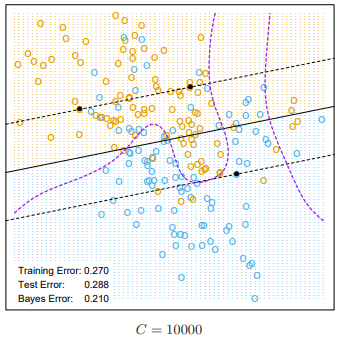
\includegraphics[width=0.4\textwidth]{img/svm_regularization_1.png}& 
             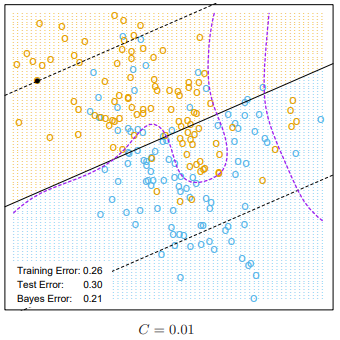
\includegraphics[width=0.4\textwidth]{img/svm_regularization_2.png}
        \end{tabular}
    \end{center}
    Чем больше $C$, тем \'{y}же разделительная полоса.
\end{frame}

\begin{frame}{Связь с другими функциями ошибки}
    \begin{itemize}
        \item На [\ref{svm_optimization}] можно взглянуть как на задачу минимизации функции ошибки $[1-M_i]_+$ с регуляризацией по $\beta$: $\underset{\beta,\beta_0}{\mathrm{min}}\; \sum_{i=1}^N [1 - M_i]_+ + \frac{\lambda}{2}\|\beta\|^2$, где $\lambda=1/C$.
        \item Для линейных классификаторов ($f(x) = x^T\beta + \beta_0$) можно рассмотреть и другие функции ошибок:
    \end{itemize}
    \includegraphicsheight{0.56}{img/svm_loss_1.png}
\end{frame}

\framedgraphic{Графики функций ошибок}{img/svm_loss_2.png}

\subsection{Kernel trick}

\begin{frame}{Двойственная задача}
\begin{itemize}
    \item Запишем двойстввенную задачу к [\ref{svm_optimization}]:
    $$
    \begin{cases}
        \mathcal{L}_D = \sum\limits_{i=1}^N\lambda_i - \frac{1}{2}\sum\limits_{i=1}^N\sum_{j=1}^N \lambda_i\lambda_jy_iy_j\langle x_i, x_j\rangle \rightarrow \min_{\lambda},\\
        0\leq \lambda_i \leq C,\\
        \sum\limits_{i=1}^N \lambda_i y_i = 0.
    \end{cases}
    $$
    \item Заметим, что лагранжиан зависит от $x_i$ только через попарные скалярные произведения $\langle x_i, x_j\rangle$. Это наводит на следующую мысль.
    \item Заменим линейное скалярное произведение $\langle x, x'\rangle$ некоторой нелинейной функцией $K(x, x')$. Это индуцирует переход в новое гильбертово пространство более высокой размерности. Решим задачу SVM в нём, получим разделяющую гиперплоскость, которая в исходном пространстве будет нелинейным многообразием. 
\end{itemize}
\end{frame}

\framedgraphic{Kernel trick}{img/svm_kernel_trick.png}

\begin{frame}{Kernel trick}
    \begin{itemize}
        \item Функция $K: X\rightarrow \mathbb{R}$ называется ядром, если $K(x, x') = \langle \psi(x), \psi(x')\rangle_H$ для некоторой функции $\psi: X\rightarrow H$, где $H$ -- гильбертово пространство.
        \item $H$ называют \textbf{спрямляющим пространством}.
        \item Можно доказать, что $K$ является ядром $\Leftrightarrow$ она симметрична и неотрицательно определена: $K(x, x') = K(x', x)$ и $\int_X\int_X K(x, x')dxdx'\geq 0$.
    \end{itemize}
\end{frame}

\begin{frame}{Примеры ядер}
\begin{itemize}
    \item $K(x, x') = (1 + \langle x, x'\rangle)^d$: полиномиальное ядро степени $d$.
    \item $K(x, x') = \tanh \kappa_1 \langle x, x'\rangle + \kappa_2$, $\kappa_1, \kappa_2 \geq 0$: нейронная сеть с сигмоидными функциями активации.
    \item $K(x, x') = \exp(-\gamma\|x-x'\|^2)$: радиальные базисные функции (см. лекцию про KNN).
\end{itemize}
\includegraphicsheight{0.5}{img/svm_kernels.png}
\end{frame}

\begin{frame}{Как работает переход в $H$. Пример.}
    \begin{itemize}
        \item Рассмотрим $K(x, x')=(1 + \langle x, x'\rangle)^d$ в $X=\mathbb{R}^2$.
        \begin{equation*}
            \begin{split}
                K(x,x') = (1 + \langle x, x'\rangle)^2 = (1 + x_1x_1' + x_2x_2')^2 =\\
                = 1 + 2x_1x_1' + 2x_2x_2' + (x_1x_1')^2 + (x_2x_2')^2 + 2x_1x_1'x_2x_2'.
            \end{split}
        \end{equation*}
        \item Отсюда видно, что $H=\mathbb{R}^6$ и $\psi(x_1, x_2) = (1, \sqrt{2}x_1, \sqrt{2}x_2, x_1^2, x_2^2, \sqrt{2}x_1x_2)$. То есть $K(x, x') = \langle \psi(x), \psi(x')\rangle_H$.
    \end{itemize}
\end{frame}

\begin{frame}{Плюсы, минусы, пдводные камни}
\begin{itemize}
    \item В основе лежит очень простая линейная идея.
    \item Легко расширяется до нелинейного решения.
    \item Одинаково хорошо работает как с табличными, так и с неструктурированными данными.
    \item Гиперпараметры (в том числе ядра) подбирать как всегда на кросс-валидации.
    \item Чувствителен к выбросам опорных объектов.
\end{itemize}
\end{frame}

\begin{frame}[allowframebreaks]
    \frametitle{Литература}
    \bibliographystyle{unsrt}
    \nocite{esl}
    \nocite{vokov}
    \bibliography{references.bib}
\end{frame}

\end{document}